\documentclass{beamer}

\usepackage{polski}
\usepackage[utf8]{inputenc}
\usepackage{soul}
\usepackage{graphicx}

\usetheme{Madrid}
\usecolortheme{beaver}

\setbeamercolor{itemize item}{fg=red}
\setbeamertemplate{itemize item}[circle]

\setbeamercolor{itemize subitem}{fg=red}
\setbeamertemplate{itemize subitem}[circle]

\setbeamercolor{itemize subsubitem}{fg=red}
\setbeamertemplate{itemize subsubitem}[circle]

\setbeamertemplate{caption}{\raggedright\textit{\insertcaption}\par}

\title[Reinforcement Learning]{Reinforcement Learning}
\subtitle{Uczenie przez ocenę zachowań w środowisku}

\author[Piotr Bielak]{Piotr Bielak (218 137)}

\institute[W8, PWr]
{Wydział Informatyki i Zarządzania\\Politechnika Wrocławska}

\date{26 lutego 2018r.}

\logo{
\includegraphics[height=1.5cm]{imgs/pwr.png}}

\begin{document}
  \titlepage

  \begin{frame}
  \frametitle{Reinforcement Learning}
  \begin{columns}
      \begin{column}{0.45\textwidth}
        \begin{itemize}
          \item{definition}
          \item{basic concepts:}
            \begin{itemize}
              \item{agent,}
              \item{environment,}
              \item{states,}
              \item{actions,}
              \item{rewards,}
              \item{etc.}
            \end{itemize}
          \item{machine learning branches:}
            \begin{itemize}
              \item{RL vs supervised learning,}
              \item{RL vs unsupervised}
            \end{itemize}
        \end{itemize}
      \end{column}

      \begin{column}{0.45\textwidth}
        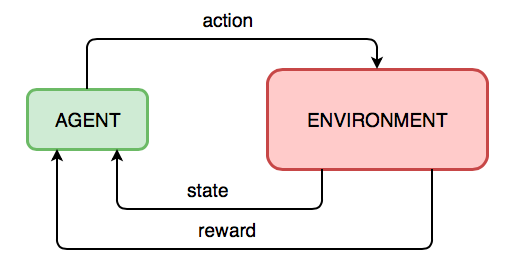
\includegraphics[width=\textwidth]{imgs/rl_model.png}
      \end{column}
  \end{columns}
\end{frame}

  \begin{frame}
  \frametitle{Theory}

  \begin{columns}
    \begin{column}{0.5\textwidth}
      Theoretical basics:
      \begin{itemize}
        \item{MDP (Markov Decision Process),}
        \item{exploitation vs exploration,}
        \item{discounted rewards,}
        \item{Bellman equation,}
        \item{essential approaches:}
          \begin{itemize}
            \item{dynamic programming,}
            \item{Monte Carlo methods,}
            \item{temporal difference (TD) learning,}
          \end{itemize}
        \item{value functions,}
        \item{policy functions,}
      \end{itemize}
    \end{column}

    \begin{column}{0.35\textwidth}
      \begin{figure}
        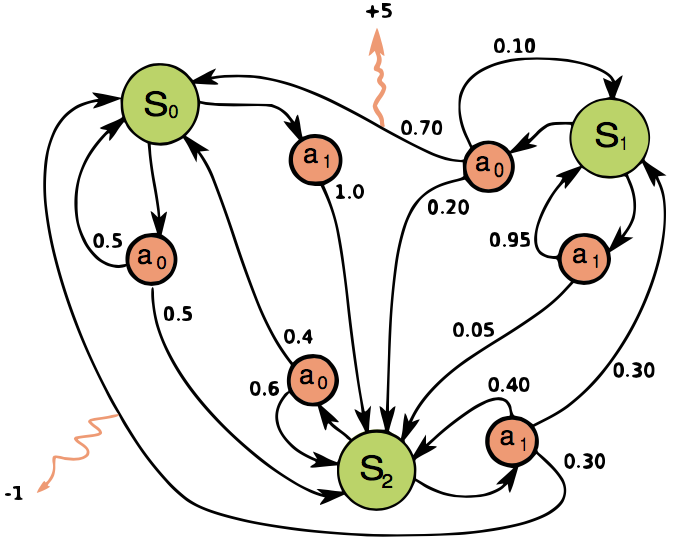
\includegraphics[width=\textwidth]{imgs/mdp.png}
        \caption{\tiny \textit{https://en.wikipedia.org/wiki/Markov\_decision\_process}}
      \end{figure}
    \end{column}
  \end{columns}

\end{frame}

  \begin{frame}
  \frametitle{Algorithms}

  \begin{columns}
    \begin{column}{0.5\textwidth}
      Most popular algorithms:
      \begin{itemize}
        \item{Q-learning,}
        \item{SARSA,}
        \item{on-policy and off-policy methods,}
        \item{actor-critic methods,}
        \item{Deep Reinforcement Learning:}
          \begin{itemize}
            \item{DQN (Deep Q-Networks),}
            \item{Deep SARSA,}
            \item{tabular approaches vs function approximators,}
          \end{itemize}
      \end{itemize}
    \end{column}

    \begin{column}{0.35\textwidth}
      \begin{figure}
        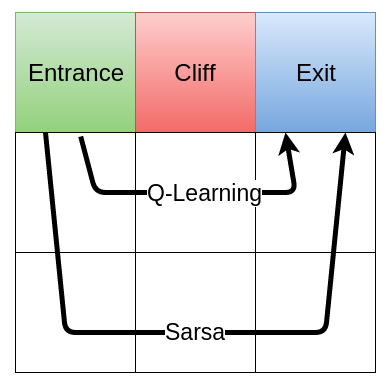
\includegraphics[width=\textwidth]{imgs/alg.png}
        \caption{\tiny \textit{https://i.stack.imgur.com/tj9DV.png}}
      \end{figure}
    \end{column}
  \end{columns}

\end{frame}

  \begin{frame}
  \frametitle{Materials}

  Books:
  \begin{itemize}
    \item{Richard S. Sutton and Andrew G. Barto, \textit{Reinforcement Learning: An Introduction}, 2017}
    \item{Csaba Szepesvari, \textit{Algorithms for Reinforcement Learning}, 2009}
  \end{itemize}

  Papers:
  \begin{itemize}
    \item{L. P. Kaelbling, M. L. Littman and A. W. Moore, \textit{Reinforcement Learning: A Survey}, 1995}
    \item{S. S. Kerrthi and B. Ravindran, \textit{A Tutorial Survey of Reinforcement Learning}, 1994}
    \item{Volodymyr Mnih et al., \textit{Human-level control through deep reinforcement learning}, 2015}
    \item{H. van Hasselt, A. Guez and D. Silver, \textit{Deep Reinforcement Learning with Double Q-learning}, 2015}
    \item{E. Morales and J. Zaragoza, \textit{An Introduction to Reinforcement Learning}, 2011}
  \end{itemize}
\end{frame}

\begin{frame}
  \frametitle{Materials}
  University courses:
  \begin{itemize}
    \item{David Silver, \textit{Reinforcement Learning}, University College London}
    \item{Stefan Riezler, \textit{Reinforcement Learning}, Universitat Heidelberg}
  \end{itemize}

  Presentations:
  \begin{itemize}
    \item{Szymon Zaręba, \textit{Reinforcement Learning}, Politechnika Wrocławska, 2017}
    \item{Witoldi Paluszyński, \textit{Reinforcement Learning}, Politechnika Wrocławska}
  \end{itemize}

\end{frame}


  \titlepage
\end{document}
